\documentclass{article}
\usepackage{graphicx}
\usepackage{amsmath}
\usepackage{amsfonts}
% or
\usepackage{amssymb}

\usepackage{tikz}
\usepackage{pgfplots}
\usepgfplotslibrary{fillbetween}
\usetikzlibrary{patterns}
\usepackage{gensymb}

\pgfplotsset{compat = newest}
\usepackage{cancel}
\usepackage[margin=1in]{geometry}
\usepackage{siunitx}
\usetikzlibrary{snakes}
\usepackage{pgflibrarysnakes}
\usetikzlibrary{decorations}

\usetikzlibrary{arrows,automata,positioning}

\usepackage{multirow}

\usepackage{listings}
\usepackage{color}

\lstset{language=c}

\begin{document}

\section{Viscosity}

\subsection{Risks}

\begin{itemize}
	\item Washing up liquid is slippy and thus would be dangerous to stand on if spilt. It should be
	cleaned up immediately after spilling to prevent this.
\end{itemize}

\subsection{Results}



\begin{center}

\begin{tabular}{|l|l|l|l|l|l|l|l|l|l|l|}
\hline
\multirow{2}{*}{\textbf{Ball Bearing}} & \multicolumn{4}{l|}{\textbf{Diameter} (\si{mm})} & 
						\multirow{2}{*}{\begin{tabular}[c]{@{}l@{}}\textbf{Rad} \\
							$\si{mm}$\end{tabular}} & 
						\multirow{2}{*}{\begin{tabular}[c]{@{}l@{}}\textbf{Vol} \\
							$\si{mm^3}$\end{tabular}} & 
						\multirow{2}{*}{\begin{tabular}[c]{@{}l@{}}\textbf{Mass} \\
						    $\si{g}$\end{tabular}} & 
						\multirow{2}{*}{\begin{tabular}[c]{@{}l@{}}\textbf{Density} \\
							$\si{kgm^{-3}}$\end{tabular}} &
						\multirow{2}{*}{\begin{tabular}[c]{@{}l@{}}\textbf{A.V. D} \\
							$\si{kgm^{-3}}$\end{tabular}} &
						\multirow{2}{*}{\begin{tabular}[c]{@{}l@{}}\textbf{A.V. R} \\
							$\si{kgm^{-3}}$\end{tabular}}						
						\\ \cline{2-5} 
                        & 1       & 2       & 3       & A.V & & & & & & \\ \hline
\multirow{2}{*}{Small}  & $4.98$  & $4.98$  & $4.98$  & $4.98$    & $2.49$ & $64.67$  & 0.51 & 7886 &
						\multirow{2}{*}{7900} & \multirow{2}{*}{2.50} \\ \cline{2-9}
                        & $4.99$  & $4.99$  & $4.99$  & $4.99$    & $2.50$ & $65.45$  & 0.51 & 7913 & & \\ \hline
\multirow{2}{*}{Medium} & $7.00$  & $6.99$  & $6.99$  & $6.99$    & $3.50$ & $179.59$ & 1.40 & 7796 & 
						\multirow{2}{*}{7796} & \multirow{2}{*}{3.50} \\ \cline{2-9} 
                        & $6.99$  & $6.99$  & $6.99$  & $6.99$    & $3.50$ & $179.59$ & 1.40 & 7796 & & \\ \hline
\multirow{2}{*}{Large}  & $10.53$ & $10.53$ & $10.53$ & $10.53$   & $5.27$ & $613.08$ & 3.56 & 5807 & 
						\multirow{2}{*}{5823} & \multirow{2}{*}{5.27}\\ \cline{2-9} 
                        & $10.54$ & $10.55$ & $10.54$ & $10.54$   & $5.27$ & $613.08$ & 3.58 & 5839 & & \\ \hline
\end{tabular}


\end{center}

\begin{center}


\begin{tabular}{|l|l|l|l|l|l|l|l|l|l|}
\hline
\multirow{2}{*}{\textbf{Ball Bearing}} & \multicolumn{4}{l|}{\textbf{Time} (\si{s})} & 
						\multicolumn{2}{l|}{\textbf{Distance}} & 
						\multirow{2}{*}{\begin{tabular}[c]{@{}l@{}}\textbf{T. Vel} \\
							$V_1 (\si{ms^{-1}})$\end{tabular}} & 
						\multirow{2}{*}{\begin{tabular}[c]{@{}l@{}}\textbf{T. Vel} \\
						    $V_2 (\si{ms^{-1}})$\end{tabular}} &
						\multirow{2}{*}{\begin{tabular}[c]{@{}l@{}}\textbf{T. Vel} \\
						    $V (\si{ms^{-1}})$\end{tabular}}
							\\ \cline{2-7} 
                        & $t_1$   & $t_2$   & A.V $t_1$             & A.V $t_2$ & $d_1$ & $d_2$ & & & \\ \hline
\multirow{3}{*}{Small}  & 0.73 & 0.91 & 
							\multirow{3}{*}{0.83} & \multirow{3}{*}{0.89} &
							\multirow{3}{*}{0.3}  & \multirow{3}{*}{0.3}  & 
							\multirow{3}{*}{0.366} & \multirow{3}{*}{0.341} &
							\multirow{3}{*}{0.354} \\ \cline{2-3} 
                        & 0.85 & 0.85 & & & & & & & \\ \cline{2-3}
                        & 0.88 & 0.90 & & & & & & & \\ \hline
\multirow{3}{*}{Medium} & 0.43 & 0.67 & 
							\multirow{3}{*}{0.49} & \multirow{3}{*}{0.49} &
							\multirow{3}{*}{0.3}  & \multirow{3}{*}{0.3}  &
							\multirow{3}{*}{0.625} & \multirow{3}{*}{0.612} &
							\multirow{3}{*}{0.619} \\ \cline{2-3}
                        & 0.48 & 0.33 & & & & & & & \\ \cline{2-3}
                        & 0.55 & 0.48 & & & & & & & \\ \hline
\multirow{3}{*}{Large}  & 0.32 & 0.34 &
							\multirow{3}{*}{0.34} & \multirow{3}{*}{0.38} &
							\multirow{3}{*}{0.3}  & \multirow{3}{*}{0.3}  &
							\multirow{3}{*}{0.882} & \multirow{3}{*}{0.789} &
							\multirow{3}{*}{0.836}
						    \\ \cline{2-3}
                        & 0.34 & 0.41 & & & & & & & \\ \cline{2-3}
                        & 0.36 & 0.39 & & & & & & & \\ \hline
\end{tabular}


\end{center}

\subsection{Analysis}

In order to calculate the viscosity, one needs to know the density:

\begin{itemize}
	\item density of liquid - 1120 \si{kgm^{-3}} - https://www.instructables.com/Density-of-Liquids-and-Materials/
\end{itemize}

In order to calculate viscosity one needs to use Stokes' law and Archimedes' principle in the following
rearrangment where $\eta$ is the viscosity of the fluid, $r$ is the radius of the bearing, $g$ is the 
gravitational feild strength, $\rho$ is the density of the bearing,
$\sigma$ is the density of the fluid and $v$ is the velocity of the bearing:
\begin{gather}
	\eta = \frac{2r^2g(\rho - \sigma)}{9v} \\
	\eta_{\text{small}} = \frac{2(2.5 \times 10^{-3})^2(9.81)(7900 - 1120)}{(9)(0.354)} = 0.262 \si{Pas} \\
	\eta_{\text{medium}} = \frac{2(3.5 \times 10^{-3})^2(9.81)(7796 - 1120)}{(9)(0.619)} = 0.288 \si{Pas} \\
	\eta_{\text{large}} = \frac{2(5.27 \times 10^{-3})^2(9.81)(5823 - 1120)}{(9)(0.836)} = 0.341 \si{Pas} \\
	\eta = \frac{0.262 + 0.288 + 0.341}{3} = 0.297 \si{Pas}\\
\end{gather}

This value is no where near the estimated 1000 \si{cP} (1 \si{Pas}) listed here: \\
https://www.newhall.co.uk/media/7440\_msds.pdf suggesting there are large inaccuracies
in the results. This is most likely down to human reaction time when recording the
times taken.

\subsubsection{Equipment}
One way in which one could increase the accuracy of results would be to use an automated way of measuring
the time the ball takes. This would remove the element of human reaction time. However, one would unlikely
be able to use light gates for this since, due to the liquid being coloured, the readings may be unreliable.

\subsubsection{Assumptions}
For these calculations we make the assumption that all the flow of the fluid is always laminar which is
not the case particularly when the ball falls close to the wall. An increase in turbulent flow increases
drag and thus makes our viscosity values larger than they should be.

\subsubsection{Caclulating Uncertanty}

\subsubsection*{Radius}

\begin{gather}
	\frac{4.99 - 4.98}{2} \times \frac{1}{4.99} = 0.2 \% \\
	\frac{7.0 - 6.99}{2} \times \frac{1}{7.0} = 0.14 \% \\
	\frac{10.55 - 10.53}{2} \times \frac{1}{10.54} = 0.19 \% \\
\end{gather}

\subsubsection*{Terminal Velocity}

\begin{gather}
	\frac{0.366 - 0.341}{2} \times \frac{1}{0.354} = 3.75 \% \\
	\frac{0.625 - 0.612}{2} \times \frac{1}{0.619} = 1.05 \% \\
	\frac{0.882 - 0.789}{2} \times \frac{1}{0.836} = 5.56 \% \\
	\frac{3.75\% + 1.05\% + 5.56\%}{3} = 3.45\%
\end{gather}

\subsubsection*{Density}

\begin{gather}
	\frac{7913 - 7886}{2} \times \frac{1}{7900} = 0.17\% \\
	\text{Because range is 0, assumed uncertanty is used:} \\
	\frac{1}{7796} = 0.01\% \\
	\frac{5839 - 5807}{2} \times \frac{1}{5823} = 0.27\%
\end{gather}

\subsubsection*{Combining}

\begin{gather}
	2 \times 0.2\% + 0.17\% + 3.75\% = 4.32\% \\
	2 \times 0.14\% + 0.01\% + 1.05\% = 1.34\% \\
	2 \times 0.19\% + 0.27\% + 5.56\% = 6.21\% \\
	\frac{4.32\% \times 0.262 + 1.34\% \times 0.288 + 6.21\% \times 0.341}{0.297} = 12.24\% \\
	0.297 \pm 12.24\%
\end{gather}

\break

\section{Stress and Strain}

\subsection{Risks}

\begin{itemize}
	\item The masses can be dangerous if dropped on someones foot and thus
		everyone should keep away from the end of the wire.

	\item Safety goggles should be worn as the wire is under tension and
		thus could be dangerous if it snapped.
\end{itemize}

\subsection{Results}

\begin{center}
    \begin{tabular}{l|l|l|l|l|l|l|l|l|l|l}
     & 1 & 2 & 3 & 4 & 5 & 6 & 7 & 8 & 9 & 10\\ \hline
     Diameter & 0.2 & 0.21 & 0.21 & 0.2 & 0.21 & 0.19 & 1.19 & 1.19 & 0.19 & 0.2
    \end{tabular}
\end{center}

\begin{equation}
	r = \frac{0.1999\si{mm}}{2} = 0.09995\si{mm} = 0.00009995 \si{m}
\end{equation}

\begin{equation}
	L = 2440\si{mm} = 2.44 \si {m}
\end{equation}


\begin{center}
    \begin{tabular}{l|l|l}
     Mass added \si{kg} & Extension \si{mm} $\pm 0.5$ & Extension $\si{m}$ \\ \hline
     0 & 0 & 0 \\
     0.1 & 0 & 0 \\
     0.2 & 0.5 & 0.0005 \\
     0.3 & 1 & 0.001\\
     0.4 & 2 & 0.002\\
     0.5 & 4 & 0.004\\
     0.6 & 10 (N.A) & 0.01 (N.A)\\
    \end{tabular}
\end{center}

\begin{center}
\begin{tikzpicture}
\begin{axis}[samples=50]

	\addplot[mark=x,smooth] coordinates {
        (0, 0.0)
        (0, 0.1)
        (0.5, 0.2)
        (1, 0.3)
        (2, 0.4)
        (4, 0.5)
        (10, 0.6)
	};

	\addplot[domain=-0.5:3,dashed] (x,0.133 * x + 0.1);

\end{axis}
\end{tikzpicture}

\end{center}

\subsection{Calculating the Youngs modulus}
\begin{gather}
	\frac{\Delta m}{\Delta \Delta l} = 0.133 \\
	E = \frac{0.133 \times 9.81 \times 2.44}{0.00009995^2 \times \pi} = 101.44 \times 10^6 = 101.44 \si{GPa}\\
\end{gather}

\subsection{Validity of Results}
The actual value for the Young's Modulus is $117 \si{GPa}$ as listed at
https://www.engineeringtoolbox.com/young-modulus-d\_417.html
which is close to our calculated value of $101.44 \si{GPa}$ showing that
the results are accurate to one significant figure.

\subsection{Wire Length}
The wire should be long since a longer wire will make the extension longer
and thus easier to read. The length of wire is directly proportional to the
extension observed.

\subsection{Measuring the Diameter}
When measuring the diameter one should measure at multiple, evenly spread, points along the wire.
At each point one should take 2 measurments at right angles to eachother. Finally, one should
take an average of all of the measurements and use it as the final diameter.

\subsection{Precision of Answers}
The ruler used to measure the extension has a low precision and thus
can only give one significant figure meaning we can only trust one
significant figure however, interpolation of data when finding
the gradient may allow one to trust a second.

\section{Gravity}

\begin{center}
    \begin{tabular}{l|l|l|l|l|l}
     $S$ & $t_1$ & $t_2$ & $t_3$ & $\overline{t}$ & ${\overline{t}}^2$\\ \hline
     0.50 & 0.314 & 0.316 & 0.315 & 0.315 & 0.0992 \\
     0.45 & 0.300 & 0.298 & 0.300 & 0.299 & 0.0894 \\
     0.40 & 0.284 & 0.283 & 0.284 & 0.284 & 0.0807 \\
     0.35 & 0.269 & 0.268 & 0.270 & 0.269 & 0.0724 \\
     0.30 & 0.245 & 0.245 & 0.245 & 0.245 & 0.0600 \\
     0.25 & 0.223 & 0.222 & 0.222 & 0.222 & 0.0493 \\
    \end{tabular}
\end{center}

\begin{center}
\begin{tikzpicture}
\begin{axis}[
	samples=50,
	xlabel={$S$ Distance},
	ylabel={$\overline{t}^2$ Time Squared}
]

	\addplot[mark=x, only marks] coordinates {
        (0.50, 0.0992)
        (0.45, 0.0894)
        (0.40, 0.0807)
        (0.35, 0.0724)
		(0.30, 0.0600)
		(0.25, 0.0493)
	};

	\addplot[domain=0.25:0.5,dashed] (x, 0.20 * x);


\end{axis}
\end{tikzpicture}

\end{center}

\subsection{Calculate Acceleration}

\begin{gather}
	S = \frac{1}{2} at^2 \\
	\frac{\Delta \hat{t}^2}{\Delta{S}} = 0.20 \\
	a = 2 \times \frac{1}{0.20} = 10 \si{ms^{-1}}
\end{gather}

\subsection{Caculating Uncertanty (6)}
\begin{center}
    \begin{tabular}{l|l|l|l|l|l}
     $S$ & Range of $t$ & $0.5 \times t$ & Actual Uncertanty & $\overline{t}$ & ${\overline{t}}^2$\\ \hline
     0.50 & 0.002 & 0.316 & 0.315 & 0.315 & 0.0992 \\
     0.45 & 0.002 & 0.298 & 0.300 & 0.299 & 0.0894 \\
     0.40 & 0.000 & 0.283 & 0.284 & 0.284 & 0.0807 \\
     0.35 & 0.002 & 0.268 & 0.270 & 0.269 & 0.0724 \\
     0.30 & 0.000 & 0.245 & 0.245 & 0.245 & 0.0600 \\
     0.25 & 0.001 & 0.222 & 0.222 & 0.222 & 0.0493 \\
    \end{tabular}
\end{center}

\begin{gather}
	R = 0.002 \\
	\frac{R}{2} = 0.001 \\
    \frac{0.001}{0.269} = 0.00372 = 0.372\% \\
	0.372\% \times 2 = 0.743\%
\end{gather}

\begin{center}
    \begin{tabular}{l|l|l|l|l|l}
     $S$ & $v_1$ & $v_2$ & $v_3$ & $\overline{v}$ & ${\overline{v}}^2$\\ \hline
     0.50 & 3.282 & 3.302 & 3.382 & 3.322 & 11.036 \\
     0.45 & 3.065 & 3.116 & 3.206 & 3.129 & 9.791 \\
     0.40 & 2.874 & 2.998 & 3.082 & 2.985 & 8.910 \\
     0.35 & 2.966 & 2.935 & 2.935 & 2.945 & 8.673 \\
	 0.30 & 2.732 & 2.680 & 2.706 & 2.706 & 7.332 \\
     0.25 & 2.433 & 2.412 & 2.476 & 2.440 & 5.954 \\
    \end{tabular}
\end{center}

\begin{center}
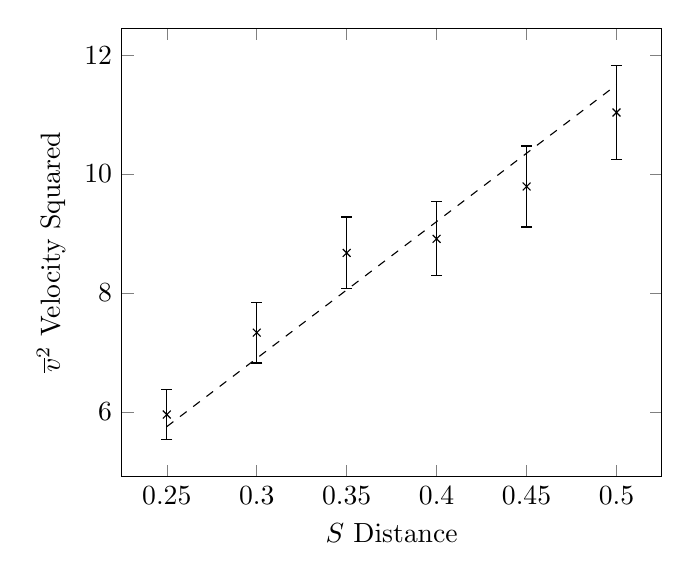
\begin{tikzpicture}
\begin{axis}[
	samples=50,
	xlabel={$S$ Distance},
	ylabel={$\overline{v}^2$ Velocity Squared}
]

	\addplot[mark=x, only marks] plot [error bars/.cd, y dir = both, y explicit] coordinates {
        (0.50, 11.036) +- (0,0.789)
        (0.45, 9.791) +- (0,0.682)
        (0.40, 8.910) +- (0,0.621)
        (0.35, 8.673) +- (0,0.604)
		(0.30, 7.332) +- (0,0.511)
		(0.25, 5.954) +- (0,0.415)
	};

	\addplot[domain=0.25:0.5,dashed] (x, 23 * x);

\end{axis}
\end{tikzpicture}
\end{center}

\subsection{Calculate Acceleration}

\begin{gather}
	S = \frac{1}{2} at^2 \\
	\frac{\Delta \overline{v}^2}{\Delta{S}} = 23 \\
	a = \frac{1}{2} \times 23 = 11.5 \si{ms^{-1}}
\end{gather}

\begin{gather}
	R = 0.208 \\
	\frac{R}{2} = 0.104 \\
    \frac{0.104}{2.985} = 0.03484 = 3.484\% \\
	3.484 \% \times 2 = 6.968 \%
\end{gather}

\subsection{Questions}
\subsubsection{Dissadvantages of Light Gates}
Compair Percentage difference, make a comment about possible error

\subsubsection{Effect of air resistance of $g$}
Air resistance will decrease the measured value of $g$ as it decreases the acceleration
by adding an opposing drag force.

\subsubsection{Graph shape}
The graph should be a straight line because there is a linear relationship between both $t^2$ and $S$ and $v^2$ and $S$,
as shown by $S = \frac{1}{2}at^2$ and $v^2 = 2aS$.

Gravity is approximately constant

\begin{center}
\begin{tikzpicture}
\begin{axis}[
	samples=50,
	xlabel={$\frac{1}{f} (\si{s})$},
	ylabel={$\lambda (\si{m})$}
]

	\addplot[mark=x, only marks] coordinates {
		(0.005, 1.660)
		(0.0025, 0.826)
		(0.001667, 0.547)
		(0.00125, 0.413)
		(0.001, 0.329)
		(0.000833, 0.275)
	};

	\addplot[domain=0.000833:0.005,dashed] (x, 332.6 * x);

\end{axis}
\end{tikzpicture}
\end{center}


\section{Resistivity}

\subsection{Results}

\subsubsection{Copper}

\begin{center}
\begin{tabular}{l|l|l|ll}
$l$ & $V$  & $I$  & $R$ &  \\ \cline{1-4}
0.1 & 0.03 & 1.43 & 0.0209 & \\
0.2 & 0.04 & 1.42 & 0.0281 & \\
0.3 & 0.05 & 1.42 & 0.0352 & \\
0.4 & 0.08 & 1.42 & 0.0563 & \\
0.5 & 0.11 & 1.41 & 0.0780 & \\
0.6 & 0.10 & 1.39 & 0.0719 & \\
0.7 & 0.20 & 1.42 & 0.1408 & \\
0.8 & 0.12 & 1.37 & 0.0876 & \\
0.9 & 0.14 & 1.38 & 0.1014 & \\
1.0 & 0.31 & 1.37 & 0.2262 & 
\end{tabular}
\end{center}

\subsubsection{Constantan}

\begin{center}
\begin{tabular}{l|ll}
$l$ & $R$ &  \\ \cline{1-2}
0.1 & 2.6 & \\
0.2 & 3.2 & \\
0.3 & 3.2 & \\
0.4 & 3.7 & \\
0.5 & 3.8 & \\
0.6 & 3.9 & \\
0.7 & 4.2 & \\
0.8 & 4.4 & \\
0.9 & 4.7 & \\
1.0 & 4.8 & 
\end{tabular}
\end{center}

\subsubsection{Diameter}

\subsubsection{Wire Diameter}

\begin{center}
\begin{tabular}{l|l|l|ll}
$d_1$ & $d_2$ & $d_3$ & $\overline{d}$ \\ \cline{1-4}
0.507 & 0.510 & 0.506 & 0.5077
\end{tabular}
\end{center}

\subsection{Calculations}

\begin{gather}
	r = \frac{\overline{d}}{2} = 0.2538 \\
	\rho = \frac{R}{l}\times A \\
	A = r^2 \pi = 0.2538^2 \pi = 0.2024 \si{mm^2} \\
	A = 0.2024 \times 10^{-6} \si{m^2}
\end{gather}


\subsubsection{Copper}

\begin{gather}
	\frac{R}{l} = m = 0.174 \\
	\rho = 0.174 \times 0.2024 \times 10^{-6} = 0.35 \times 10^{-7} \si{\Omega m}
\end{gather}

\subsubsection{Constantan}

\begin{gather}
	\frac{R}{l} = m = \frac{\Delta y}{\Delta x} = \frac{19.5}{0.75} = 26 \\
	\rho = 26 \times 0.2024 \times 10^{-6} = 5.2624 \times 10 ^{-6} \\
	\rho = 5.3 \times 10^{-6} \si{\Omega m}
\end{gather}

\subsection{Error}

\begin{gather}
	\%err_d = \frac{0.005}{0.5077} = 0.0098 = 0.98\% \\
	\%err_{d^2} = 2 \times \%err_d = 1.97\%
\end{gather}

\subsubsection{Copper}

\begin{gather}
	\text{Worse Line Of Best Fit (WLOBF):} \\
	m_\text{wlobf} = 0.12 \\
	\text{\% difference in gradient:} \\
	\%err_m = \frac{0.174 - 0.12}{0.174} = 0.3103 = 31\% \\
	\%err_{\rho} = \%err_m + \%err_d = 32.97\%
\end{gather}
\\
The actual resistivity of Copper\footnote{according
to http://hyperphysics.phy-astr.gsu.edu/hbase/Tables/rstiv.html on 2021-03-29}:
$0.168 \times 10^{-7}$ 

\begin{gather}
	\%diff_{\rho} = \left | \frac{0.168 - 0.35}{0.168} \right | = 1.083 = 108.3\% > 31\%
\end{gather}
Due to the the \% difference being larger than the estimated \% error, the
results are not valid and there was likely systematic error as the whole \%
difference can not be explained by error in the equipment alone

\subsubsection{Constantan}

\begin{gather}
	\text{Worse Line Of Best Fit (WLOBF):} \\
	m_\text{wlobf} = \frac{16.5}{0.8} = 20.625 \\
	\text{\% difference in gradient:} \\
	\%err_m = \frac{26 - 20.625}{26} = 0.2067 = 20.67\% \\
	\%err_{\rho} = \%err_m + \%err_d = 22.64\%
\end{gather}
\\
The actual resistivity of Constantan\footnote{according
to http://hyperphysics.phy-astr.gsu.edu/hbase/Tables/rstiv.html on 2021-03-29}:
$0.49 \times 10^{-6}$ 

\begin{gather}
	\%diff_{\rho} = \left | \frac{0.49 - 5.3}{0.49} \right | = 9.816 = 981.6\% > 22.64\%
\end{gather}
Due to the the \% difference being much larger than the estimated \% error, the
results are not valid and there was likely systematic error as the whole \%
difference can not be explained by error in the equipment alone

\subsection{Questions}

\subsubsection{Explain why the graph doesn't cross the origin}
The resistance of the connecting wires and the contact resistance
of the connection between the crocodile clips and the Constantan or
Copper offset the graph preventing the resistance from ever being 0.

\subsubsection{Explain how you might change the apparatus to calculate your value for the resistivity with greater resolution}
Using higher resolution apparatus to measure the diameter of the wire and use
a higher resolution voltmeter and ammeter

\subsubsection{Explain why plotting a graph improves your accuracy}
Plotting a graph allows one to quickly and easily take an average value
by calculating the gradient of a line of best fit. Plotting a graph
also makes it easier to spot anomalous results.

\subsubsection{Explain why you need to use a wire to find the resistivity of a metal and explain what shape of sample would be suitable for a plastic}
Wire is used because of it's constant cross section and long thin shape.
the long thin shape helps to increase the resistance of the wire making it
easier to measure. For plastics, the sample should be very short to reduce
the resistance as much as possible. This is done because the resistance of
plastic is so high it's not easily measurable.

\subsubsection{Identify the sources of uncertainty in this experiment. Consider the accuracy (percentage difference) of your result and comment on the effect the uncertainies might have had}
Contact resistance is not necessarily constant, temperature of the wire

\subsubsection{Explain why the current through the wire should be small}
A large current results in a greater amount of heat from the wire; this
alters the resistive characteristics of the wire making the results inaccurate

\break

\section{EMF and Internal Resistance}

\subsection{Results}

\begin{center}
\begin{tabular}{l|ll}
$p.d\, (\si{V})$   & $I\, (\si{A})$  &  \\ \cline{1-2}
0.110 & 0.532 & \\
0.490 & 0.367 & \\
0.706 & 0.277 & \\
0.821 & 0.229 & \\
0.888 & 0.201 & \\
0.949 & 0.177 & \\
1.008 & 0.152 & \\
1.118 & 0.107 & \\
\end{tabular}
\end{center}



\subsection{Calculations}

\begin{gather}
	r = -m = - \frac{\Delta y}{\Delta x} = \frac{1.08}{49} = 0.02204 \si{k\Omega} \\
	r = 22.0 \si{\Omega}
\end{gather}
\\
Given to 3 significant figures because all original readings are 3 significant figures.

\subsection{Accuracy}
The results are likely accurate because $22.0 \si{\Omega}$ is within the manufacturing
tollerence of the $22 \si{\Omega}$ resistor that was placed in series with the cell.

\subsection{Questions}

\subsubsection{When the internal resistance is large in comparison to the
	external resistance, the terminal potential difference falls to a small value.
	This is used to make high voltage supplies safe for use in a laboratory.
	Explain how this makes the supply safe.}

Making the internal resistance of a high voltage power supply much larger
than the human bodies natural resistance (roughly $100 \si{k\Omega}$ for dry
skin) greatly reduces the potential difference across the human body thus
preventing a large enough current from flowing through the human body to do any
significant damage.

\subsubsection{It should not matter whether the voltmeter is connected across $R$
	or across the cell. This is partly because of the low resistance of the
	ammeter. Explain why. }

Due to the ammeters negligible resistance, the potential difference across the
ammeter is also negligible and thus can be ignored making the potential
difference across the cell and $R$ effectively the same.

\subsubsection{The intercept of your graph will be very close to the true value
	for the emf of the cell. Account for any difference.}
Errors in graph plotting and the voltmeter not having an infinite resistance.

\subsubsection{Explain any difference between your value for r and the
	manufacturer’s value.}
The cell itself has an internal resistance ontop of the extern resister we
added and the external resister has a 5\% manufacturing tollerence.

\break

\section{Wavelength of Laser Light}

\subsection{Results}

\begin{center}
\begin{tabular}{l|l|l|l|l|l|ll}
  & $x_1$ & $x_2$ & $x$ & $D$ & $\theta$        & $\lambda$         & \\ \cline{1-7}
1 & 610   & 404   & 103 & 506 & $11.51 \degree$ & 6.3875            & \\
2 & 703   & 303   & 200 & 506 & $21.57 \degree$ & $\times 10^{-17}$ &
\end{tabular}
\end{center}

\subsection{Error}

\begin{gather}
	\%diff = \left | \frac{6.35 - 6.3875}{6.35} \right | = 0.0059 = 0.59 \%
\end{gather}

\subsection{Questions}

\subsubsection{State the advantages of using laser light in this experiment}
Lasers are bright making the maxima easy to see even for a large value of $D$.
Lasers are monochromatic and coherent also helping to increase the clarity of
the maximum.

\subsubsection{Explain why a metre ruler is suitable for measuring the distance
	in the experiment}
Using a metre ruler gives a resolution of 1\si{mm} which gives a small enough
uncertanty for the values of $x$ and $D$ for the purpose of this experiment.

\subsubsection{Suppose that a white light laser were possible. Describe what
	the diffraction maxima would look like}

Which light is a mixture of multiple frequencies which each diffract
differently. This results in the colours separating at the maxima making
the inner part of the maxima look slightly blue and the outer part slightly
red.

\break

\section{Photoelectric Effect}

\begin{gather}
	hf = \varphi + \frac{1}{2} mv^2 \\
	eVs = hf - \varphi \\
	Vs = \frac{h}{e}f - \frac{\varphi}{e}
\end{gather}
\end{document}
